\sectionlink{経路積分の短期講義}\label{app:A}

経路積分は、特に非自明な位相を持つ曲面上で、量子論を表す強力な手段である。ここで示す入門は、現代の場の理論の教科書で読者が目にするものと同様である。経路積分と Hilbert 空間形式の関係や、経路積分内での演算子方程式の使用など、必要となるいくつかの考え方を強調するために、本付録を設けた。

\subsectionlink{ボソン場}

まず、一自由度で Hamiltonian $\hat H(\hat p,\hat q)$ を持つ量子力学の問題を考える。ここで
\begin{equation}
[\hat q,\hat p]=i\hbar.
\tag{A.1.1}\label{eq:A.1.1}
\end{equation}
本付録では一貫して、ハットで演算子を表す。関心のある基本的な量は、時間 $T$ の間に、ある $q$ 固有状態から別の固有状態へ発展する振幅
\begin{equation}
\langle q_f|\exp(-i\hat HT/\hbar)|q_i\rangle
\tag{A.1.2}\label{eq:A.1.2}
\end{equation}
である。

場の理論では、一般に Heisenberg 表示を使うと便利である。この表示で演算子の時間依存性は
\begin{equation}
\hat A(t)=\exp(i\hat Ht/\hbar)\hat A\exp(-i\hat Ht/\hbar)
\tag{A.1.3}\label{eq:A.1.3}
\end{equation}
である。状態 $\lvert q,t\rangle$ は $\hat q(t)$ の固有状態であり、
\begin{equation}
\hat q(t)|q,t\rangle=|q,t\rangle q.
\tag{A.1.4}\label{eq:A.1.4}
\end{equation}
$t=0$ の Schrödinger 固有状態で書けば、
\begin{equation}
|q,t\rangle=\exp(i\hat Ht/\hbar)|q\rangle.
\tag{A.1.5}\label{eq:A.1.5}
\end{equation}
この記法では、遷移振幅\hyperref[eq:A.1.2]{(A.1.2)}は $\langle q_f,T|q_i,0\rangle$ である。

\begin{figure}[tbp]
\centering
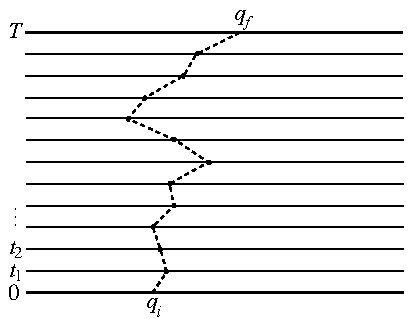
\includegraphics[width=0.8\linewidth]{figures/fig_A_1.pdf}
\caption{時間刻みに分解した遷移振幅。破線は区分的に線形な経路を示唆しており、これは経路積分を定義する多くの方法の一つである。}
\label{fig:A.1}
\end{figure}

状態の完全系を挿入すると、遷移振幅を、中間のある時刻 $t$ に系が通過しうるすべての状態 $q$ にわたる、コヒーレントな和として書ける。
\begin{equation}
\langle q_f,T|q_i,0\rangle
=\int dq\,\langle q_f,T|q,t\rangle\langle q,t|q_i,0\rangle.
\tag{A.1.6}\label{eq:A.1.6}
\end{equation}
図\ref{fig:A.1}のように時間区間をさらに $N$ 個の刻みに分け、
\begin{equation}
t_m=m\epsilon,\qquad\epsilon=T/N
\tag{A.1.7}\label{eq:A.1.7}
\end{equation}
とし、各中間時刻に対応して状態の完全系を挿入する。
\begin{equation}
\langle q_f,T|q_i,0\rangle
=\int dq_{N-1}\cdots dq_1
\prod_{m=0}^{N-1}\langle q_{m+1},t_{m+1}|q_m,t_m\rangle.
\tag{A.1.8}\label{eq:A.1.8}
\end{equation}
Schrödinger 形式に戻し、中間の運動量についての積分を導入する。
\begin{equation}
\begin{aligned}
\langle q_{m+1},t_{m+1}|q_m,t_m\rangle
&=\langle q_{m+1}|\exp(-i\hat H\epsilon/\hbar)|q_m\rangle\\
&=\int dp_m\,\langle q_{m+1}|p_m\rangle
\langle p_m|\exp(-i\hat H\epsilon/\hbar)|q_m\rangle.
\end{aligned}
\tag{A.1.9}\label{eq:A.1.9}
\end{equation}
交換関係を用いれば、$\hat H$ は常に、すべての $\hat p$ を左、すべての $\hat q$ を右に置いて書けるので、
\begin{equation}
\langle p_m|\hat H(\hat p,\hat q)|q_m\rangle
=H(p_m,q_m)\langle p_m|q_m\rangle.
\tag{A.1.10}\label{eq:A.1.10}
\end{equation}
これを用いて式\hyperref[eq:A.1.9]{(A.1.9)}の行列要素を評価する。指数関数を展開すると、$\hat q$ が $\hat p$ の左にある $\epsilon^2$ 以上の次数の項が生じるが、これらを捨てる。この次数までで、$\langle q_{m+1},t_{m+1}|q_m,t_m\rangle$ は
\begin{equation}
\begin{aligned}
&\int dp_m\,\exp[-iH(p_m,q_m)\epsilon/\hbar]
\langle q_{m+1}|p_m\rangle\langle p_m|q_m\rangle\\
&\quad=\int\frac{dp_m}{2\pi\hbar}
\exp\left\{-\frac i\hbar
[H(p_m,q_m)\epsilon-p_m(q_{m+1}-q_m)]
+O(\epsilon^2)\right\}
\end{aligned}
\tag{A.1.11}\label{eq:A.1.11}
\end{equation}
となる。したがって、
\begin{equation}
\begin{aligned}
\langle q_f,T|q_i,0\rangle
\approx{}&\int\frac{dp_{N-1}}{2\pi\hbar}\,dq_{N-1}\cdots
\frac{dp_1}{2\pi\hbar}\,dq_1\frac{dp_0}{2\pi\hbar}\\
&\times\exp\left\{-\frac i\hbar
\sum_{m=0}^{N-1}
[H(p_m,q_m)\epsilon-p_m(q_{m+1}-q_m)]\right\}\\
\longrightarrow{}&\int[dp\,dq]\,
\exp\left\{\frac i\hbar\int_0^Tdt\,[p\dot q-H(p,q)]\right\}.
\end{aligned}
\tag{A.1.12}\label{eq:A.1.12}
\end{equation}
最終行では形式的な $\epsilon\to0$ の極限をとったので、積分は、指定した $q(T)$ と $q(0)$ を持つすべての経路 $p(t),q(t)$ にわたる。これは Hamiltonian 経路積分（または汎関数積分）であり、Hamiltonian 形式の作用を $S$ として、$\exp(iS/\hbar)$ で重みを付けた位相空間の経路についての和である。

$p(t)$ について積分しよう。まず、積分は位相が停留する点によって支配されると近似する。
\begin{equation}
0=\frac{\partial}{\partial p}[p\dot q-H(p,q)]
=\dot q-\frac{\partial}{\partial p}H(p,q).
\tag{A.1.13}\label{eq:A.1.13}
\end{equation}
$p$ を $q,\dot q$ で解き、$L=p\dot q-H$ を思い出すと、停留位相近似は
\begin{equation}
\langle q_f,T|q_i,0\rangle
=\int[dq]\exp\left[\frac i\hbar\int_0^Tdt\,L(q,\dot q)\right]
\tag{A.1.14}\label{eq:A.1.14}
\end{equation}
を与える。しばしば運動量積分は Gaussian 型で、$\hat H=\tfrac12\hat p^2+V(\hat q)$ であり、その場合には、測度 $[dq]$ に吸収できる規格化を除き、停留位相近似は厳密である。実際、一般にも同じことができる。$p$ と $\dot q$ の関係\hyperref[eq:A.1.13]{(A.1.13)}が局所的なので、停留位相近似への補正も局所的であり、$[dq]$ が各中間時刻での独立した積分の積であるという本質的な性質を損なわずに、その定義に吸収できるからである。結果\hyperref[eq:A.1.14]{(A.1.14)}は Lagrangian 経路積分である。これは、今度は Lagrangian 形式の作用を $S$ として、$\exp(iS/\hbar)$ で重みを付けた配位空間のすべての経路についての積分である。

古典極限を議論するために $\hbar$ を残しておいた。$\hbar\to0$ では、位相が停留する経路、$\delta S/\delta q(t)=0$ が積分を支配する。これは確かに古典的な運動方程式である。以後は $\hbar=1$ とする。

以上の導出は、明らかに多成分の $q^i$ に一般化できる。空間座標 $\mathbf x$ を離散化して極限をとるか、$\mathbf x$ 依存性を Fourier モードで展開すれば、場の量子論は常に無限個の $q$ で書ける。したがって、上の経路積分表示の導出は、ボソン場の理論にも適用できる。

経路積分の公式の導出では、連続極限 $\epsilon\to0$ をかなり発見的に扱った。繰り込み理論は、この極限操作を研究するものであり、かなりよく理解されている。Lagrangian が一定の条件（繰り込み可能性）を満たし、極限をとる際に Lagrangian の係数（裸の結合定数）を適切に変化させれば、極限は存在する。結果は、途中で選ばなければならないさまざまな事柄、たとえば Hamiltonian 内の演算子の順序、測度の厳密な定義、正則化の違い（たとえば図で示唆した区分的線形経路の極限と、Fourier モードの周波数カットオフとの違い）に依存しない。\footnote[1]{別の例として、場のスケールを自由に変えてよい。その Jacobian は形式的には各点での Jacobian の積であり、その対数は各点での局所的な式の和になる。正則化すると、これは裸の結合定数の移動にすぎない。}これらは局所的な効果なので、すべて裸の結合定数に吸収できる。実際に明示的に評価するのは、少数の Gaussian 経路積分だけである。経路積分は主として、演算子方程式や縫い合わせの関係など、一般的な結果を導くために用いる。

\subsubsectionlink*{Hilbert 空間形式との関係}

経路積分から出発し、それを切り開くことで、理論の Hilbert 空間を回復できる。式\hyperref[eq:A.1.6]{(A.1.6)}で、各振幅を経路積分として書くと、
\begin{equation}
\begin{aligned}
&\int[dq]_{q_i,0}^{q_f,T}
\exp\left(i\int_0^Tdt\,L\right)\\
&\quad=\int dq\int[dq]_{q,t}^{q_f,T}
\exp\left(i\int_t^Tdt\,L\right)
\int[dq]_{q_i,0}^{q,t}
\exp\left(i\int_0^tdt\,L\right).
\end{aligned}
\tag{A.1.15}\label{eq:A.1.15}
\end{equation}
すなわち、$[0,T]$ 上の経路積分は、$[0,t]$ と $[t,T]$ 上の別々の経路積分と、$q(t)$ に関する通常の積分とに分かれる。経路の境界条件は上下の添字で示した。$T\geq t\geq0$ という制限に注意しよう。中間の積分は、任意の完全な状態系についての和に置き換えてもよい。この切断（逆にいえば縫い合わせ）の原理は、弦理論に現れる非自明な位相の曲面で特に有用である。そのような曲面は、さまざまな閉曲線に沿って切り開ける。異なる選び方は、一つの振幅に対して異なる Hilbert 空間表示を与える。これは世界面双対性として知られている。

ここで、$0<t<T$ において因子 $q(t)$ を追加で挿入した経路積分を考えよう。切断関係\hyperref[eq:A.1.15]{(A.1.15)}を用いると、
\begin{equation}
\begin{aligned}
\int[dq]_{q_i,0}^{q_f,T}\exp(iS)q(t)
&=\int dq\,\langle q_f,T|q,t\rangle\,q\,\langle q,t|q_i,0\rangle\\
&=\int dq\,\langle q_f,T|\hat q(t)|q,t\rangle
\langle q,t|q_i,0\rangle\\
&=\langle q_f,T|\hat q(t)|q_i,0\rangle.
\end{aligned}
\tag{A.1.16}\label{eq:A.1.16}
\end{equation}
したがって、汎関数積分の $q(t)$ は、行列要素の $\hat q(t)$ に翻訳される。二つの挿入の積 $q(t)q(t')$（単なる積分変数なので $q(t')q(t)$ と等しい）について、$t,t'$ がともに $[0,T]$ にあるとすると、同じ方法で
\begin{equation}
\int[dq]_{q_i,0}^{q_f,T}\exp(iS)q(t)q(t')
=\langle q_f,T|\mathrm T[\hat q(t)\hat q(t')]|q_i,0\rangle
\tag{A.1.17}\label{eq:A.1.17}
\end{equation}
が得られる。ここで $\mathrm T$ は時間順序積
\begin{equation}
\mathrm T[\hat A(t)\hat B(t')]
=\theta(t-t')\hat A(t)\hat B(t')
+\theta(t'-t)\hat B(t')\hat A(t)
\tag{A.1.18}\label{eq:A.1.18}
\end{equation}
を表す。経路積分は無限小の時間切片を順次つないで構成されるため、経路積分中の二つ以上の挿入は、常に行列要素中の演算子の時間順序積に対応する。

運動方程式は $\delta S/\delta q(t)=0$ である。これが経路積分の中でどのように働くかを見よう。他の挿入 $\mathcal F$ を伴う経路積分で、この方程式を考える。
\begin{equation}
\begin{aligned}
\int[dq]_{q_i,0}^{q_f,T}\exp(iS)\frac{\delta S}{\delta q(t)}\mathcal F
&=-i\int[dq]_{q_i,0}^{q_f,T}
\left[\frac{\delta}{\delta q(t)}\exp(iS)\right]\mathcal F\\
&=i\int[dq]_{q_i,0}^{q_f,T}\exp(iS)
\frac{\delta\mathcal F}{\delta q(t)}.
\end{aligned}
\tag{A.1.19}\label{eq:A.1.19}
\end{equation}
第二行では部分積分した。\footnote[2]{汎関数微分は
\[
\frac{\delta}{\delta q(t)}q(t')=\delta(t-t')
\]
と定義される。これは通常の微分
\[
\frac1\epsilon\frac{\partial}{\partial q_m},
\qquad m=t/\epsilon
\]
の極限とみなせる。特に、通常の微分と同様に、汎関数微分を部分積分できる。}
$\mathcal F$ の中の場がどれも時刻 $t$ にない場合、右辺は消え、運動方程式は経路積分内で成立する。そこで、運動方程式は演算子方程式として成り立つという。これは今後広く用いる手法である。演算子方程式とは、その方程式に含まれる場と位置が一致する他の場を持たない、任意の経路積分に挿入したときに成立する方程式である。Hilbert 空間の言葉に翻訳すると、他の挿入 $\mathcal F$ によって任意の初期状態と終状態を設定できるので、これは、演算子方程式は一般の行列要素に対して成り立つはずだという通常の概念に対応する。

時刻 $t$ に追加の挿入が存在すると、経路積分内の演算子方程式は、デルタ関数の源の項を追加した形でのみ成立する。たとえば $\mathcal F=q(t')\cdots$ とし、$t'$ は $t$ の近く、「$\cdots$」の他の場は遠くにあるとしよう。式\hyperref[eq:A.1.19]{(A.1.19)}は
\begin{equation}
\left\langle q(t')\frac{\delta S}{\delta q(t)}\cdots\right\rangle
=i\langle\delta(t-t')\cdots\rangle
\tag{A.1.20}\label{eq:A.1.20}
\end{equation}
となる。これは、場の積の期待値についての運動方程式である Schwinger--Dyson 方程式の例である。同じ結果を演算子方程式として書けば、
\begin{equation}
q(t')\frac{\delta S}{\delta q(t)}=i\delta(t-t').
\tag{A.1.21}\label{eq:A.1.21}
\end{equation}

具体例として、調和振動子をとる。
\begin{align}
S&=\frac12\int dt\,(\dot q^2-\omega^2q^2),
\tag{A.1.22a}\label{eq:A.1.22a}\\
\frac{\delta S}{\delta q(t)}&=-\ddot q(t)-\omega^2q(t).
\tag{A.1.22b}\label{eq:A.1.22b}
\end{align}
導いた演算子方程式は
\begin{equation}
\left(\frac{\partial^2}{\partial t^2}+\omega^2\right)q(t)=0
\tag{A.1.23}\label{eq:A.1.23}
\end{equation}
および
\begin{equation}
\left(\frac{\partial^2}{\partial t^2}+\omega^2\right)
q(t)q(t')=-i\delta(t-t')
\tag{A.1.24}\label{eq:A.1.24}
\end{equation}
である。Hilbert 空間の言葉では、これらは
\begin{equation}
\begin{aligned}
\left(\frac{\partial^2}{\partial t^2}+\omega^2\right)\hat q(t)&=0,\\
\left(\frac{\partial^2}{\partial t^2}+\omega^2\right)
\mathrm T[\hat q(t)\hat q(t')]&=-i\delta(t-t')
\end{aligned}
\tag{A.1.25a}\label{eq:A.1.25a}
\end{equation}
となる。第一式は場の演算子の Heisenberg 方程式であり、第二式のデルタ関数は、時間順序積の階段関数に時間微分が作用することから生じる。
\begin{equation}
\begin{aligned}
\left(\frac{\partial^2}{\partial t^2}+\omega^2\right)
\mathrm T[\hat q(t)\hat q(t')]
={}&\mathrm T\left\{[\ddot{\hat q}(t)+\omega^2\hat q(t)]\hat q(t')\right\}\\
&+\delta(t-t')[\dot{\hat q}(t),\hat q(t)]\\
={}&0-i\delta(t-t').
\end{aligned}
\tag{A.1.26}\label{eq:A.1.26}
\end{equation}

\subsubsectionlink*{Euclid 経路積分}

Schrödinger の言葉では、時間順序積\hyperref[eq:A.1.17]{(A.1.17)}は
\begin{equation}
\langle q_f|
\exp[-i\hat H(T-t_>)]\hat q\,
\exp[-i\hat H(t_>-t_<)]\hat q\,
\exp[-i\hat Ht_<]|q_i\rangle
\tag{A.1.27}\label{eq:A.1.27}
\end{equation}
である。$t_>$ は $t,t'$ の大きい方、$t_<$ は小さい方である。時間刻みを順次つないで振幅を作るという経路積分の性質により、\hyperref[eq:A.1.27]{(A.1.27)}のような振幅で $H$ に掛かる時間差は常に正である。すなわち、$\exp(-iH\Delta t)$ に現れるのは正の $\Delta t$ だけである。ここで、すべての時間を複素平面で一様に回転し、$0\leq\theta\leq\pi$ の任意の位相について $t\to e^{-i\theta}t$ として解析接続する。指数の実部は $-E\sin\theta\,\Delta t$ であり、$E$ は中間状態のエネルギーである。安定な系では Hamiltonian は下に有界なので、中間状態についての和は問題なく収束し、特異点には遭遇しない。接続された振幅は明確に定義される。

実数 $u$ に対して $t=-iu$ と時間を純虚数にとると、これまで調べた Minkowski 振幅に対する Euclid 振幅が定義される。
\begin{equation}
\left\langle q_f,u\left|
\mathrm T\left[\prod_a\hat q(u_a)\right]\right|q_i,0\right\rangle_{\mathrm E}
\tag{A.1.28}\label{eq:A.1.28}
\end{equation}
は、
\begin{equation}
\left\langle q_f,t\left|
\mathrm T\left[\prod_a\hat q(t_a)\right]\right|q_i,0\right\rangle
\tag{A.1.29}\label{eq:A.1.29}
\end{equation}
を $t=-iu$ へ接続したものとして定義する。Euclid の場合にも経路積分表示の導出を繰り返せるが、結果はきわめて簡単であり、作用中の $t$ を $-iu$ に置き換えるだけである。
\begin{equation}
\begin{aligned}
&\left\langle q_f,U\left|
\mathrm T\left[\prod_a\hat q(u_a)\right]\right|q_i,0\right\rangle_{\mathrm E}\\
&\qquad=\int[dq]_{q_i,0}^{q_f,U}
\exp\left[\int_0^Udu\,L(q,i\partial_uq)\right]\prod_aq(u_a).
\end{aligned}
\tag{A.1.30}\label{eq:A.1.30}
\end{equation}
Euclid 経路積分の重みは、慣習的に $\exp(-S_{\mathrm E})$ と定義するので、Euclid 作用には負号が入る。
\begin{equation}
S_{\mathrm E}=\int du\,L_{\mathrm E}(q,\partial_uq)
=-\int du\,L(q,i\partial_uq).
\tag{A.1.31}\label{eq:A.1.31}
\end{equation}
作用の指数関数が振動せずに減衰するため、Euclid 経路積分の方が通常は明確に定義される。その後、解析接続によって Minkowski の行列要素が得られる。本書の本文で主に扱うのは Euclid 経路積分であり、弦の S 行列を表すために用いる。

しばしば関心があるのは、たとえば
\begin{equation}
\operatorname{Tr}\exp(-\hat HU)=\sum_i\exp(-E_iU)
\tag{A.1.32}\label{eq:A.1.32}
\end{equation}
のようなトレースである。和は $\hat H$ のすべての固有ベクトルにわたり、$E_i$ は対応する固有値である。$q$ 基底ではトレースは
\begin{equation}
\begin{aligned}
\int dq\,\langle q|\exp(-\hat HU)|q\rangle
&=\int dq\,\langle q,U|q,0\rangle_{\mathrm E}\\
&=\int dq\int[dq]_{q,0}^{q,U}\exp(-S_{\mathrm E})\\
&=\int[dq]_{\mathrm P}\exp(-S_{\mathrm E})
\end{aligned}
\tag{A.1.33}\label{eq:A.1.33}
\end{equation}
となる。最終行の $[dq]_{\mathrm P}$ は、$[0,U]$ 上のすべての周期的な経路についての積分を表す。興味深い変形として、すべての反周期的な経路についての積分がある。
\begin{equation}
\begin{aligned}
\int[dq]_{\mathrm A}\exp(-S_{\mathrm E})
&=\int dq\int[dq]_{-q,0}^{q,U}\exp(-S_{\mathrm E})\\
&=\int dq\,\langle q,U|-q,0\rangle_{\mathrm E}\\
&=\int dq\,\langle q,U|\hat R|q,0\rangle_{\mathrm E}\\
&=\operatorname{Tr}[\exp(-\hat HU)\hat R].
\end{aligned}
\tag{A.1.34}\label{eq:A.1.34}
\end{equation}
ここで $\hat R$ は $q$ を $-q$ にする反射演算子である。境界条件をひねること、たとえば周期的なものを反周期的なものに置き換えることは、トレース内に演算子を挿入することに等しいとわかる。$\hat R^2=1$ なので、固有値は $\pm1$ である。周期的な経路積分と反周期的な経路積分の平均をとると、$\hat R=+1$ の空間に射影する $\tfrac12(1+\hat R)$ が挿入される。
\begin{equation}
\frac12(\text{周期的}+\text{反周期的})
=\sum_{R_i=+1}\exp(-E_iU).
\tag{A.1.35}\label{eq:A.1.35}
\end{equation}
同様に、$\tfrac12(\text{周期的}-\text{反周期的})$ は $\hat R=-1$ の空間上のトレースを与える。

小さいが、ときに混乱を招く点がある。$\hat A$ が Hermite 演算子であっても、Euclid の Heisenberg 演算子 $\hat A(u)=\exp(\hat Hu)\hat A\exp(-\hat Hu)$ は
\begin{equation}
\hat A(u)^\dagger=\hat A(-u)
\tag{A.1.36}\label{eq:A.1.36}
\end{equation}
を満たすため、一般には Hermite ではない。このため、Euclid 随伴
\begin{equation}
\overline{\hat A(u)}=\hat A(-u)^\dagger
\tag{A.1.37}\label{eq:A.1.37}
\end{equation}
を定義すると便利である。Schrödinger 描像の Hermite 演算子は、Euclid の Heisenberg 描像では Euclid 自己随伴になる。

\subsubsectionlink*{図式と行列式}

図式展開は、経路積分から容易に得られる。この話題は現代の場の理論の教科書でよく扱われている。ここでは、本文で使ういくつかの結果だけを導く。記法を明確にするために場の理論へ移り、$q(t)$ を実スカラー場 $\phi(t,\mathbf x)$ に置き換える。自由な作用
\begin{equation}
\frac12\int d^dx\,\phi(x)\Delta\phi(x)
\tag{A.1.38}\label{eq:A.1.38}
\end{equation}
から出発する。ここで $\Delta$ はある微分演算子である。具体的に Euclid の場合をとり、源 $J(x)$ を持つ経路積分を考える。
\begin{equation}
\begin{aligned}
Z[J]&=\left\langle\exp\left[i\int d^dx\,J(x)\phi(x)\right]\right\rangle\\
&=\int[d\phi]\exp\left[
-\frac12\int d^dx\,\phi(x)\Delta\phi(x)
+i\int d^dx\,J(x)\phi(x)\right].
\end{aligned}
\tag{A.1.39}\label{eq:A.1.39}
\end{equation}
これは Euclid の Green 関数の生成汎関数である。$J(x)$ に関する汎関数微分をとると、積分内に因子 $i\phi(x)$ が降りてくる。$\phi$ を $\phi+i\Delta^{-1}J$ にずらすと平方完成され、
\begin{equation}
\begin{aligned}
Z[J]&=Z[0]\exp\left[
-\frac12\int d^dx\,d^dy\,J(x)\Delta^{-1}(x,y)J(y)\right]\\
&=Z[0]\exp\left[
\frac12\int d^dx\,d^dy\,\Delta^{-1}(x,y)
\frac{\delta^2}{\delta\phi(x)\delta\phi(y)}\right]\\
&\qquad\times
\left.\exp\left[i\int d^dx\,J(x)\phi(x)\right]\right|_{\phi=0}
\end{aligned}
\tag{A.1.40}\label{eq:A.1.40}
\end{equation}
が残る。第二行では、各 $\phi$ 微分が $iJ$ になる。$\phi$ の任意の汎関数 $\mathcal F$ は
\begin{equation}
\mathcal F[\phi]
=\int[dJ]\exp\left[i\int d^dx\,J(x)\phi(x)\right]f[J]
\tag{A.1.41}\label{eq:A.1.41}
\end{equation}
と書ける。$f[J]$ は $\mathcal F$ の（汎関数の）Fourier 変換である。線形性から
\begin{equation}
\langle\mathcal F\rangle
=Z[0]\left.
\exp\left[
\frac12\int d^dx\,d^dy\,\Delta^{-1}(x,y)
\frac{\delta^2}{\delta\phi(x)\delta\phi(y)}\right]\mathcal F[\phi]
\right|_{\phi=0}
\tag{A.1.42}\label{eq:A.1.42}
\end{equation}
が得られる。指数関数を展開すると、$\mathcal F$ 内の場の対を縮約するすべての方法、すなわち図式展開が生成される。また、$\mathcal F$ が因子の積 $\mathcal F_1\mathcal F_2\cdots$ であるとき、
\begin{equation}
\frac{\delta}{\delta\phi(x)}
=\frac{\delta}{\delta\phi_1(x)}
+\frac{\delta}{\delta\phi_2(x)}+\cdots
\tag{A.1.43}\label{eq:A.1.43}
\end{equation}
と分けられる。ここで $\delta/\delta\phi_i$ は $\mathcal F_i$ にだけ作用する。自己縮約は、項
\begin{equation}
\frac{\delta^2}{\delta\phi_i(x)\delta\phi_i(y)}
\qquad(i\text{ について和をとらない})
\tag{A.1.44}\label{eq:A.1.44}
\end{equation}
である。

次に全体の因子 $Z[0]$ を考える。$\Delta$ は自己随伴と仮定し、その固有関数 $\Phi_i(x)$ の完全系で $\phi(x)$ を展開する。
\begin{equation}
\phi(x)=\sum_i\phi_i\Phi_i(x).
\tag{A.1.45}\label{eq:A.1.45}
\end{equation}
ここで
\begin{align}
\Delta\Phi_i(x)&=\lambda_i\Phi_i(x),
\tag{A.1.46a}\label{eq:A.1.46a}\\
\int d^dx\,\Phi_i(x)\Phi_j(x)&=\delta_{ij}.
\tag{A.1.46b}\label{eq:A.1.46b}
\end{align}
経路積分の測度を
\begin{equation}
[d\phi]=\prod_i d\phi_i
\tag{A.1.47}\label{eq:A.1.47}
\end{equation}
で定義する。すると、
\begin{equation}
\begin{aligned}
\langle1\rangle
&=\prod_i\left[\int d\phi_i\exp\left(-\frac12\phi_i^2\lambda_i\right)\right]\\
&=\prod_i\left(\frac{2\pi}{\lambda_i}\right)^{1/2}\\
&=\left(\det\frac{\Delta}{2\pi}\right)^{-1/2}.
\end{aligned}
\tag{A.1.48}\label{eq:A.1.48}
\end{equation}
固有値の積は、適切に正則化し繰り込む必要がある。$\langle1\rangle$ は通常、単に $(\det\Delta)^{-1/2}$ と書かれる。$\Delta$ のスケール変換は $\phi$ のスケール変換に等しく、その Jacobian は裸の結合定数に吸収できるからである。（自由場の理論で繰り込まれる唯一の「結合」は、Lagrangian 密度の c 数定数となる。これが例の中で現れるのを見ることになる。）

以上の議論はすべて、多成分の $q^i$ や $\phi^i$ に容易に拡張できる。興味のある一例は複素スカラー場である。これは二つの実スカラーに $\phi=2^{-1/2}(\phi^1+i\phi^2)$ と分けられ、測度は $[d\phi\,d\phi^*]\equiv[d\phi^1\,d\phi^2]$ である。複素場の場合、\hyperref[eq:A.1.48]{(A.1.48)}は
\begin{equation}
\int[d\phi\,d\phi^*]\exp\left(-\int d^dx\,\phi^*\Delta\phi\right)
=(\det\Delta)^{-1}
\tag{A.1.49}\label{eq:A.1.49}
\end{equation}
となる。同様に、二つの実場について
\begin{equation}
\int[d\phi^1\,d\phi^2]\exp\left(i\int d^dx\,\phi^1\Delta\phi^2\right)
=(\det\Delta)^{-1}
\tag{A.1.50}\label{eq:A.1.50}
\end{equation}
を得る。これは、デルタ関数の積分
\begin{equation}
\int_{-\infty}^{\infty}dx\int_{-\infty}^{\infty}dy\,\exp(i\lambda xy)
=2\pi\int_{-\infty}^{\infty}dx\,\delta(\lambda x)
=\frac{2\pi}{\lambda}
\tag{A.1.51}\label{eq:A.1.51}
\end{equation}
の汎関数版である。

\subsubsectionlink*{一つの例}

例として、調和振動子の Euclid 遷移振幅を調べる。
\begin{align}
\langle q_f,U|q_i,0\rangle_{\mathrm E}
&=\int[dq]_{q_i,0}^{q_f,U}\exp(-S_{\mathrm E}),
\tag{A.1.52a}\label{eq:A.1.52a}\\
S_{\mathrm E}
&=\frac12\int_0^Udu\,[(\partial_uq)^2+\omega^2q^2]+S_{\mathrm{ct}}.
\tag{A.1.52b}\label{eq:A.1.52b}
\end{align}
$S_{\mathrm{ct}}$ はカットオフに依存する部分で、後で決定する。これを評価するため、$q$ の「古典的」な部分を分離する。
\begin{equation}
q(u)=q_{\mathrm{cl}}(u)+q'(u).
\tag{A.1.53}\label{eq:A.1.53}
\end{equation}
ここで
\begin{align}
-\ddot q_{\mathrm{cl}}(u)+\omega^2q_{\mathrm{cl}}(u)&=0,
\tag{A.1.54a}\label{eq:A.1.54a}\\
q_{\mathrm{cl}}(0)=q_i,\qquad q_{\mathrm{cl}}(U)&=q_f.
\tag{A.1.54b}\label{eq:A.1.54b}
\end{align}
このとき、$q'$ の境界条件は
\begin{equation}
q'(0)=q'(U)=0
\tag{A.1.55}\label{eq:A.1.55}
\end{equation}
となり、作用は
\begin{equation}
S_{\mathrm E}=S_{\mathrm{cl}}(q_i,q_f)+S'+S_{\mathrm{ct}}
\tag{A.1.56}\label{eq:A.1.56}
\end{equation}
と分かれる。ここで
\begin{align}
S_{\mathrm{cl}}(q_i,q_f)
&=\frac12\int_0^Udu\,[(\partial_uq_{\mathrm{cl}})^2+\omega^2q_{\mathrm{cl}}^2]
\notag\\
&=\omega\frac{(q_i^2+q_f^2)\cosh\omega U-2q_iq_f}{2\sinh\omega U},
\tag{A.1.57a}\label{eq:A.1.57a}\\
S'&=\frac12\int_0^Udu\,[(\partial_uq')^2+\omega^2q'{}^2].
\tag{A.1.57b}\label{eq:A.1.57b}
\end{align}
振幅は
\begin{equation}
\langle q_f,U|q_i,0\rangle
=\exp[-S_{\mathrm{cl}}(q_i,q_f)-S_{\mathrm{ct}}]
\int[dq']_{0,0}^{0,U}\exp(-S')
\tag{A.1.58}\label{eq:A.1.58}
\end{equation}
となる。

境界条件\hyperref[eq:A.1.55]{(A.1.55)}を満たす $\Delta=-\partial_u^2+\omega^2$ の固有関数の完全系で展開する。
\begin{align}
f_j(u)&=\left(\frac2U\right)^{1/2}\sin\frac{j\pi u}U,
\qquad\lambda_j=\frac{j^2\pi^2}{U^2}+\omega^2,
\tag{A.1.59a}\label{eq:A.1.59a}\\
\det\frac{\Delta}{2\pi}
&=\prod_{j=1}^{\infty}\frac{j^2\pi^2+\omega^2U^2}{2\pi U^2}.
\tag{A.1.59b}\label{eq:A.1.59b}
\end{align}
この無限積は発散する。Pauli--Villars 正則化は、これを定義する簡単な方法である。非常に高い周波数 $\Omega$ を持つ正則化用振動子の振幅で割る。
\begin{equation}
\det\frac{\Delta}{2\pi}
\xrightarrow{\text{正則化}}
\prod_{j=1}^{\infty}\frac{j^2\pi^2+\omega^2U^2}{j^2\pi^2+\Omega^2U^2}.
\tag{A.1.60}\label{eq:A.1.60}
\end{equation}
$j$ が小さいとき、\hyperref[eq:A.1.60]{(A.1.60)}の各項は、乗法的な定数を除いて\hyperref[eq:A.1.59b]{(A.1.59b)}と同じであり、$j$ が大きいときには積が収束する。積\hyperref[eq:A.1.60]{(A.1.60)}の値は
\begin{equation}
\frac{\Omega\sinh\omega U}{\omega\sinh\Omega U}
\tag{A.1.61}\label{eq:A.1.61}
\end{equation}
である。これは $\sinh$ の標準的な無限積表示から従う。$U$ に関して正しい極と零点を持ち、$U\to0$ で正しい値をとることに注意すれば、結果\hyperref[eq:A.1.61]{(A.1.61)}を推測できる。

$\Omega\to\infty$ で消えない項だけを残すと、
\begin{equation}
\begin{aligned}
\langle q_f,U|q_i,0\rangle\longrightarrow{}
&\left(\frac{\omega}{2\sinh\omega U}\right)^{1/2}\\
&\times\exp\left[
-S_{\mathrm{cl}}(q_i,q_f)+\frac12(\Omega U-\ln\Omega)-S_{\mathrm{ct}}\right].
\end{aligned}
\tag{A.1.62}\label{eq:A.1.62}
\end{equation}
$\Omega\to\infty$ で有限な答えを得るには、まず Lagrangian $L_{\mathrm{ct}}$ に項 $\tfrac12\Omega$ を含め、\hyperref[eq:A.1.62]{(A.1.62)}の線形発散を相殺する必要がある。すなわち、演算子「1」に対して線形に発散する裸の結合定数がある。量子力学の問題で繰り込みが必要なのは奇妙に思えるかもしれないが、べきの数え上げは場の量子論と完全に共通している。対数発散は波動関数の繰り込みである。有限な規格化を定めるには、経路積分表示\hyperref[eq:A.1.62]{(A.1.62)}を、$U\to\infty$ における正準的な結果と比較する。この極限では基底状態 $\lvert0\rangle$ だけが寄与するため、状態の完全系を挿入すれば $U\to\infty$ の振幅を容易に評価できる。
\begin{equation}
\begin{aligned}
\langle q_f,U|q_i,0\rangle
&\longrightarrow\langle q_f|0\rangle\langle0|q_i\rangle\exp(-E_0U)\\
&=\left(\frac\omega\pi\right)^{1/2}
\exp\left[-\frac\omega2(q_f^2+q_i^2+U)\right].
\end{aligned}
\tag{A.1.63}\label{eq:A.1.63}
\end{equation}
一方、経路積分表示\hyperref[eq:A.1.62]{(A.1.62)}は
\begin{equation}
\langle q_f,U|q_i,0\rangle\longrightarrow
\omega^{1/2}\exp\left[
-\frac\omega2(q_f^2+q_i^2+U)
+\frac12(\Omega U-\ln\Omega)-S_{\mathrm{ct}}\right]
\tag{A.1.64}\label{eq:A.1.64}
\end{equation}
となる。したがって、
\begin{equation}
S_{\mathrm{ct}}
=\frac12\left[\int_0^Udu\,\Omega\right]
-\frac12\ln\frac\Omega\pi
\tag{A.1.65}\label{eq:A.1.65}
\end{equation}
および
\begin{equation}
\langle q_f,U|q_i,0\rangle
=\left(\frac{\omega}{2\pi\sinh\omega U}\right)^{1/2}
\exp(-S_{\mathrm{cl}})
\tag{A.1.66}\label{eq:A.1.66}
\end{equation}
を得る。これは正しい結果である。

\subsectionlink{フェルミオン場}

基本的なフェルミオンの量子系、すなわち上昇演算子 $\hat\chi$ と下降演算子 $\hat\psi$ を持つ二つの状態 $\lvert\uparrow\rangle,\lvert\downarrow\rangle$ を考える。
\begin{align}
\hat\psi|\downarrow\rangle&=0,\qquad
\hat\chi|\downarrow\rangle=|\uparrow\rangle,
\tag{A.2.1a}\label{eq:A.2.1a}\\
\hat\psi|\uparrow\rangle&=|\downarrow\rangle,\qquad
\hat\chi|\uparrow\rangle=0,
\tag{A.2.1b}\label{eq:A.2.1b}\\
\{\hat\psi,\hat\chi\}&=1,\qquad\hat\psi^2=\hat\chi^2=0.
\tag{A.2.1c}\label{eq:A.2.1c}
\end{align}
振幅は、$\hat\chi,\hat\psi$ の古典的な対応物についての経路積分で表される。これらは反交換する c 数、または Grassmann 変数であり、Grassmann 代数
\begin{equation}
\{\chi_m,\psi_n\}=\{\chi_m,\chi_n\}=\{\psi_m,\psi_n\}=0
\tag{A.2.2}\label{eq:A.2.2}
\end{equation}
の要素 $\chi_m,\psi_m$ である。

Grassmann 変数に対する積分には、自然な概念である Berezin 積分がある。$\theta$ が Grassmann 変数なら $\theta^2=0$ であるから、$\theta$ の最も一般的な関数は $a+\theta b$ の形であることに注意しよう。
\begin{equation}
\int d\theta=0,\qquad
\int d\theta\,\theta=-\int\theta\,d\theta=1
\tag{A.2.3}\label{eq:A.2.3}
\end{equation}
と定義する。より一般的な式の積分は、積分の線形性を要求し、$d\theta$ がすべての Grassmann 変数と反交換すると定義することで定まる。定義\hyperref[eq:A.2.3]{(A.2.3)}の意義は、全微分の積分がゼロになることにある。
\begin{equation}
\int d\theta\,\frac d{d\theta}(a+\theta b)
=\int d\theta\,b=0.
\tag{A.2.4}\label{eq:A.2.4}
\end{equation}
複数の Grassmann 変数では、積分は
\begin{equation}
\int d\theta_1\cdots d\theta_n\,f(\theta)=c
\tag{A.2.5}\label{eq:A.2.5}
\end{equation}
であり、$c$ は $f$ の Taylor 展開の最高次の項の係数である。
\begin{equation}
f(\theta)=\cdots+\theta_n\theta_{n-1}\cdots\theta_1c.
\tag{A.2.6}\label{eq:A.2.6}
\end{equation}
ボソンの経路積分の議論を振り返ると、そこで用いた通常の積分の性質、すなわち線形性、積分順序の変更に対する（符号を除いた）不変性、部分積分は、すべて Berezin 積分にも成り立つことがわかる。\footnote[3]{$\int d\theta$ を通常の意味での積分と考えるのは有用でない。これは単に、$\theta$ の関数から複素数への線形写像である。通常の積分と非常に多くの性質を共有するため、積分の記法は便利な覚え書きとなる。}

ボソンの議論にできるだけ忠実に従うため、形式的に $\hat\psi$ の固有状態となる状態を定義すると便利である。
\begin{align}
|\psi\rangle&=|\downarrow\rangle+|\uparrow\rangle\psi,
\tag{A.2.7a}\label{eq:A.2.7a}\\
\hat\psi|\psi\rangle&=|\psi\rangle\psi.
\tag{A.2.7b}\label{eq:A.2.7b}
\end{align}
$\langle\psi|$ を
\begin{equation}
\langle\psi|\psi'\rangle=\psi-\psi'
\tag{A.2.8}\label{eq:A.2.8}
\end{equation}
を満たすように定義する。右辺は Dirac のデルタ関数の Grassmann 版である。通常のデルタ関数と同じ性質
\begin{equation}
(\psi-\psi')f(\psi)=(\psi-\psi')f(\psi')
\tag{A.2.9}\label{eq:A.2.9}
\end{equation}
および
\begin{equation}
\int d\psi\,(\psi-\psi')f(\psi)=f(\psi')
\tag{A.2.10}\label{eq:A.2.10}
\end{equation}
を、任意の $f(\psi)$ に対して持つ。状態 $\langle\psi|$ は、符号が逆の左固有状態である。
\begin{equation}
\langle\psi|\hat\psi=-\psi\langle\psi|.
\tag{A.2.11}\label{eq:A.2.11}
\end{equation}
これは、両辺と一般の状態 $\lvert\psi'\rangle$ との内積をとれば確かめられる。また、
\begin{equation}
\int|\psi\rangle\,d\psi\,\langle\psi|=1
\tag{A.2.12}\label{eq:A.2.12}
\end{equation}
にも注意しよう。任意の状態 $\langle\psi'|$ と $\lvert\psi''\rangle$ の間の行列要素をとり、Grassmann 積分を評価すれば、これを確認できる。

デルタ関数は積分表示
\begin{equation}
-\int d\chi\,\exp[\chi(\psi'-\psi)]
=\psi-\psi'=\langle\psi|\psi'\rangle
\tag{A.2.13}\label{eq:A.2.13}
\end{equation}
を持つ。内積\hyperref[eq:A.2.8]{(A.2.8)}を $\psi'$ のべきで展開すると、
\begin{equation}
\langle\psi|\downarrow\rangle=\psi,\qquad
\langle\psi|\uparrow\rangle=-1
\tag{A.2.14}\label{eq:A.2.14}
\end{equation}
を得る。したがって、
\begin{equation}
\begin{aligned}
\langle\psi|\hat\chi|\psi'\rangle
&=\langle\psi|\uparrow\rangle\\
&=-\int d\chi\,\chi\exp[\chi(\psi'-\psi)].
\end{aligned}
\tag{A.2.15}\label{eq:A.2.15}
\end{equation}
さらに、$\lvert\psi\rangle$ が $\hat\psi$ の固有状態であることを使うと、
\begin{equation}
-\langle\psi|f(\hat\chi,\hat\psi)|\psi'\rangle
=\int d\chi\,f(\chi,\psi')\exp[\chi(\psi'-\psi)]
\tag{A.2.16}\label{eq:A.2.16}
\end{equation}
を得る。これは、$\hat\psi$ を右に置いて書くという処方のもとで、任意の関数 $f$ に成り立つ。

これでボソンの場合の議論をなぞることができる。完全性関係\hyperref[eq:A.2.12]{(A.2.12)}を用いて、時間刻みを順次つなぎ合わせると、
\begin{equation}
\begin{aligned}
\langle\psi_f,T|\psi_i,0\rangle
\approx{}&-\int d\chi_0\,d\psi_1\,d\chi_1\cdots
d\psi_{N-1}\,d\chi_{N-1}\\
&\times\exp\sum_{m=0}^{N-1}
[-iH(\chi_m,\psi_m)\epsilon-\chi_m(\psi_{m+1}-\psi_m)]\\
\longrightarrow{}&\int[d\chi\,d\psi]\,
\exp\left\{\int_0^Tdt\,[-\chi\dot\psi-iH(\chi,\psi)]\right\}
\end{aligned}
\tag{A.2.17}\label{eq:A.2.17}
\end{equation}
を得る。積分表示の扱いにくい符号は、Grassmann 積分の順序を逆にすることで相殺された。典型的なフェルミオンの Hamiltonian は $\hat H=m\hat\chi\hat\psi$ である。対応する Lagrangian は $L=i\chi\dot\psi-H$ である。このような一階の Lagrangian では、Hamiltonian 形式と Lagrangian 形式は一致し、結果\hyperref[eq:A.2.17]{(A.2.17)}は Lagrangian 経路積分でもある。

この系には、二つの有用な内積がある。
\begin{align}
\text{(A)}:\quad
&\langle\uparrow|\uparrow\rangle
=\langle\downarrow|\downarrow\rangle=1,\qquad
\langle\uparrow|\downarrow\rangle
=\langle\downarrow|\uparrow\rangle=0,
\tag{A.2.18a}\label{eq:A.2.18a}\\
\text{(B)}:\quad
&\langle\uparrow|\downarrow\rangle
=\langle\downarrow|\uparrow\rangle=1,\qquad
\langle\uparrow|\uparrow\rangle
=\langle\downarrow|\downarrow\rangle=0.
\tag{A.2.18b}\label{eq:A.2.18b}
\end{align}
内積(A)は正定値で、$\hat\psi^\dagger=\hat\chi$ を与える。通常の物理的な振動子に対する内積である。内積(B)は正ではなく、$\hat\psi$ と $\hat\chi$ を Hermite にする。第4章で議論したように、これは Faddeev--Popov ゴースト系に適した内積である。経路積分の導出は内積の選び方に依存しなかったが、関係式\hyperref[eq:A.2.14]{(A.2.14)}は、内積に応じて $\langle\psi|$ の基底状態による展開を決める。

ボソンの場合の議論はすべて、フェルミオンの経路積分にも適用できる。導出は、複数の Fermi 振動子や場の理論へ容易に拡張される。繰り込み理論も、ボソンの経路積分と同じように働く。フェルミオンの経路積分も切断関係を満たし、それは単に、累次積分\hyperref[eq:A.2.17]{(A.2.17)}の一つを最後まで取っておくことに相当する。経路積分中への $\psi(t),\chi(t)$ の挿入は、やはり行列要素中に対応する演算子を与え、複数の挿入はやはり時間順序積となる。経路積分の挿入
\begin{equation}
\psi(t)\psi(t')=-\psi(t')\psi(t)
\tag{A.2.19}\label{eq:A.2.19}
\end{equation}
は、演算子
\begin{equation}
\mathrm T[\hat\psi(t)\hat\psi(t')]
\equiv\theta(t-t')\hat\psi(t)\hat\psi(t')
-\theta(t'-t)\hat\psi(t')\hat\psi(t)
\tag{A.2.20}\label{eq:A.2.20}
\end{equation}
になる。時間順序積の定義に負号が現れることに注意しよう。運動方程式や Euclid への接続はボソンの場合と同様に働くが、一つ重要な違いがある。一般の演算子 $\hat A$ を考える。
\begin{equation}
\hat A|i\rangle=|j\rangle A_{ji}.
\tag{A.2.21}\label{eq:A.2.21}
\end{equation}
$i,j$ は $\downarrow,\uparrow$ を走る。$\hat A|\psi\rangle$ を基底状態で展開すると、
\begin{equation}
\begin{aligned}
\int d\psi\,\langle\psi|\hat A|\psi\rangle
&=A_{\downarrow\downarrow}-A_{\uparrow\uparrow}\\
&=\operatorname{Tr}[(-1)^{\hat F}\hat A]
\end{aligned}
\tag{A.2.22}\label{eq:A.2.22}
\end{equation}
が得られる。フェルミオン数 $\hat F$ は、$\lvert\downarrow\rangle$ で偶数、$\lvert\uparrow\rangle$ で奇数になるように定義した。特に、
\begin{equation}
\int d\psi\,\langle\psi,U|\psi,0\rangle
=\operatorname{Tr}[(-1)^{\hat F}\exp(-\hat HU)].
\tag{A.2.23}\label{eq:A.2.23}
\end{equation}
ボソンの場合の結果\hyperref[eq:A.1.33]{(A.1.33)}、\hyperref[eq:A.1.34]{(A.1.34)}と異なり、周期的な経路積分は $(-1)^{\hat F}$ で重みを付けたトレースを与え、反周期的な経路積分は単純なトレースを与える。

Feynman 図はボソンの場合と同じだが、行列式の結果は異なる。
\begin{equation}
\langle1\rangle
=\int[d\psi\,d\chi]\exp\left(\int d^dx\,\chi\Delta\psi\right)
\tag{A.2.24}\label{eq:A.2.24}
\end{equation}
を考えよう。ここでも場の理論の記法に切り替えた。$\psi$ を $\Delta$ の固有関数で、$\chi$ を $\Delta^T$ の固有関数で展開する。
\begin{align}
\psi(x)&=\sum_i\psi_i\Psi_i(x),\qquad
\chi(x)=\sum_i\chi_i\Upsilon_i(x),
\tag{A.2.25a}\label{eq:A.2.25a}\\
\Delta\Psi_i(x)&=\lambda_i\Psi_i(x),\qquad
\Delta^T\Upsilon_i(x)=\lambda_i\Upsilon_i(x),
\tag{A.2.25b}\label{eq:A.2.25b}\\
\int d^dx\,\Upsilon_i(x)\Psi_j(x)&=\delta_{ij}.
\tag{A.2.25c}\label{eq:A.2.25c}
\end{align}
$[d\psi\,d\chi]=\prod_i d\psi_i\,d\chi_i$ と定義する。すると、
\begin{equation}
\begin{aligned}
\langle1\rangle
&=\prod_i\left[\int d\psi_i\,d\chi_i\exp(\lambda_i\chi_i\psi_i)\right]\\
&=\prod_i\lambda_i\\
&=\det\Delta.
\end{aligned}
\tag{A.2.26}\label{eq:A.2.26}
\end{equation}
同様に、一つの場 $\psi$ について
\begin{equation}
\int[d\psi]\exp\left(\int d^dx\,\psi\Delta\psi\right)
=(\det\Delta)^{1/2}
\tag{A.2.27}\label{eq:A.2.27}
\end{equation}
が得られる。ここで $\Delta$ は反対称でなければならない。これらのフェルミオンの経路積分は、対応するボソンの積分の逆数にほかならない。

有限次元の積分では、$2\pi$ に注意する必要がある。
\begin{equation}
\int_{-\infty}^{\infty}dx\int_{-\infty}^{\infty}dy\,
\exp(2\pi i\lambda xy)
=\frac1\lambda
=\left[\int d\psi\int d\chi\,\exp(\lambda\chi\psi)\right]^{-1}.
\tag{A.2.28}\label{eq:A.2.28}
\end{equation}
興味深いことに、汎関数行列式ではもっと大まかに扱える。場のスケール変換によって、これらの因子を除けるからである。実際には、ボソンの経路積分は行列式の絶対値を与える。一方、フェルミオンの経路積分は、測度中の Grassmann 因子の厳密な順序に依存する符号を伴う行列式を与える。符号は手で決めることにする。\footnote[4]{細かい点として、世界面の理論がパリティ非対称な場合には、経路積分の位相さえも曖昧になる。この場合、Euclid 随伴は時間反転（これはパリティ反転と Euclid 回転の組合せに等しい）を含むため、$\Delta$ が Hermite でないことが要点である。代わりに Hermite 演算子 $\Delta^\dagger\Delta$ の行列式をとらなければならず、これでは $\Delta$ の行列式は位相を除いてしか決まらない。たとえば第10.7節でこの状況に出会い、位相を整合的に定義できるか確認する必要が生じる。}

$\Delta$ がゼロ固有値を持つと、経路積分はフェルミオンの場合には消え、ボソンの場合には発散する。実際の例で見るように、これが起きるときには常に十分な理由があり、関心のある積分には、有限な結果を与える適切な挿入が含まれる。

Berezin 積分についての有用な結果がある。定義から、$\theta'=\theta a$ ならば $d\theta'=a^{-1}d\theta$ が従う。すなわち、Jacobian はボソンの場合の逆数である。より一般に、ボソン変数 $x_i$ と Grassmann 変数 $\theta_j$ があり、一般的な変数変換 $x'_i(x,\theta),\theta'_j(x,\theta)$ を行うと、測度の無限小変換には余分な負号がある。
\begin{equation}
\delta(d^mx\,d^n\theta)
=d^mx\,d^n\theta
\left(\sum_i\frac{\partial}{\partial x_i}\delta x_i
-\sum_j\frac{\partial}{\partial\theta_j}\delta\theta_j\right).
\tag{A.2.29}\label{eq:A.2.29}
\end{equation}

\subsectionlink*{演習}
\addcontentsline{toc}{subsection}{演習問題}

\subsubsection*{演習A.1}\label{ex:A.1}
\begin{enumerate}
\item[(a)] 調和振動子の経路積分\hyperref[eq:A.1.33]{(A.1.33)}を、$[dq]_{\mathrm P}$ を周期的な固有関数の集合で展開して評価せよ（すでに得た遷移関数の結果を左辺に代入する方法は用いない）。状態についての和\hyperref[eq:A.1.32]{(A.1.32)}を明示的に評価した結果と比較せよ。
\item[(b)] 反周期的な経路積分\hyperref[eq:A.1.34]{(A.1.34)}についても同じことを行え。
\end{enumerate}

\subsubsection*{演習A.2}\label{ex:A.2}
同じ周波数の調和振動子を二つ考え、複素座標 $q=2^{-1/2}(q_1+iq_2)$ を作る。適切なモード展開を用いて、$[0,U]$ 上の次の経路積分を評価せよ。
\[
\int[dq\,dq^*]_\theta\exp(-S_{\mathrm E}).
\]
ここで積分は、$q(U)=q(0)e^{i\theta}$ を満たすすべての経路にわたる。ここでも状態について和をとって得た答えと比較せよ。この際、振動子の複素結合 $a_1\pm ia_2$ を作ると便利である。これは演習A.1の、より風変わりな版であり、オービフォールドなど、さまざまな弦理論に現れる。

\subsubsection*{演習A.3}\label{ex:A.3}
二次元の自由スカラー場 $X$ を、作用
\[
S=\frac1{4\pi\alpha'}\int d^2\sigma\,
\left(\partial_1X\partial_1X+\partial_2X\partial_2X+m^2X^2\right)
\]
で考える。両座標が周期的な場合の経路積分を評価せよ。
\[
0\leq\sigma_1\leq2\pi,\qquad0\leq\sigma_2\leq T.
\]
［空間依存性を Fourier モードで展開すると、答えは調和振動子のトレースの無限積の形になる。］

\subsubsection*{演習A.4}\label{ex:A.4}
円周上の自由粒子
\[
H=-\frac12\frac{\partial^2}{\partial\phi^2}
\]
を考える。経路積分によって $\langle\phi_f,T|\phi_i,0\rangle$ を評価せよ。円周を巻く回数によって区別される、位相的に非同値な経路があることに注意せよ。

\subsubsection*{演習A.5}\label{ex:A.5}
演習A.1のフェルミオン版を考える。周期関数または反周期関数の完全系を用いて、フェルミオンの経路積分\hyperref[eq:A.2.23]{(A.2.23)}と対応する反周期的な経路積分を評価し、状態についての和と比較せよ。
